% Options for packages loaded elsewhere
\PassOptionsToPackage{unicode}{hyperref}
\PassOptionsToPackage{hyphens}{url}
%
\documentclass[
  13pt,
  ignorenonframetext,
]{beamer}
\usepackage{pgfpages}
\setbeamertemplate{caption}[numbered]
\setbeamertemplate{caption label separator}{: }
\setbeamercolor{caption name}{fg=normal text.fg}
\beamertemplatenavigationsymbolsempty
% Prevent slide breaks in the middle of a paragraph
\widowpenalties 1 10000
\raggedbottom
\setbeamertemplate{part page}{
  \centering
  \begin{beamercolorbox}[sep=16pt,center]{part title}
    \usebeamerfont{part title}\insertpart\par
  \end{beamercolorbox}
}
\setbeamertemplate{section page}{
  \centering
  \begin{beamercolorbox}[sep=12pt,center]{section title}
    \usebeamerfont{section title}\insertsection\par
  \end{beamercolorbox}
}
\setbeamertemplate{subsection page}{
  \centering
  \begin{beamercolorbox}[sep=8pt,center]{subsection title}
    \usebeamerfont{subsection title}\insertsubsection\par
  \end{beamercolorbox}
}
\AtBeginPart{
  \frame{\partpage}
}
\AtBeginSection{
  \ifbibliography
  \else
    \frame{\sectionpage}
  \fi
}
\AtBeginSubsection{
  \frame{\subsectionpage}
}
\usepackage{amsmath,amssymb}
\usepackage{iftex}
\ifPDFTeX
  \usepackage[T1]{fontenc}
  \usepackage[utf8]{inputenc}
  \usepackage{textcomp} % provide euro and other symbols
\else % if luatex or xetex
  \usepackage{unicode-math} % this also loads fontspec
  \defaultfontfeatures{Scale=MatchLowercase}
  \defaultfontfeatures[\rmfamily]{Ligatures=TeX,Scale=1}
\fi
\usepackage{lmodern}
\usetheme[]{Antibes}
\usecolortheme{seahorse}
\ifPDFTeX\else
  % xetex/luatex font selection
\fi
% Use upquote if available, for straight quotes in verbatim environments
\IfFileExists{upquote.sty}{\usepackage{upquote}}{}
\IfFileExists{microtype.sty}{% use microtype if available
  \usepackage[]{microtype}
  \UseMicrotypeSet[protrusion]{basicmath} % disable protrusion for tt fonts
}{}
\makeatletter
\@ifundefined{KOMAClassName}{% if non-KOMA class
  \IfFileExists{parskip.sty}{%
    \usepackage{parskip}
  }{% else
    \setlength{\parindent}{0pt}
    \setlength{\parskip}{6pt plus 2pt minus 1pt}}
}{% if KOMA class
  \KOMAoptions{parskip=half}}
\makeatother
\usepackage{xcolor}
\newif\ifbibliography
\setlength{\emergencystretch}{3em} % prevent overfull lines
\providecommand{\tightlist}{%
  \setlength{\itemsep}{0pt}\setlength{\parskip}{0pt}}
\setcounter{secnumdepth}{-\maxdimen} % remove section numbering
\usepackage[spanish, es-tabla]{babel}
\usepackage{graphicx}
\usepackage{caption}
\usepackage{hyperref}
\usepackage{float}
\usepackage[export]{adjustbox}
\usepackage{xcolor}
\usepackage{bookmark}
\IfFileExists{xurl.sty}{\usepackage{xurl}}{} % add URL line breaks if available
\urlstyle{same}
\hypersetup{
  pdftitle={Tutorial para instalación de R},
  pdfauthor={Santiago Ortúzar},
  hidelinks,
  pdfcreator={LaTeX via pandoc}}

\title{Tutorial para instalación de R}
\author{Santiago Ortúzar}
\date{Viernes 1 de abril de 2022}
\institute{\href{mailto:saortuza@uc.cl}{\nolinkurl{saortuza@uc.cl}} \and Estadística
Descriptiva en R \and Prof.~Alejandro González \and Universidad Alberto
Hurtado}

\begin{document}
\frame{\titlepage}

\section{Introducción a R}\label{introducciuxf3n-a-r}

\begin{frame}{¿Qué es R?}
\phantomsection\label{quuxe9-es-r}
\begin{itemize}
\item
  R es un software para el procesamiento, administración y análisis de
  datos cuantitativos.\footnote<.->{Clase basada en material utilizado
    en clases por el prof. Ignacio Madero y otros textos de consulta que
    se mencionan al final.}
\item
  En las sesiones de ayudantía, nuestros objetivos serán:

  \begin{itemize}
  \item
    Familiarizarnos con algunas operaciones básicas en R para manipular
    datos;
  \item
    Generar análisis estadísticos simples (además de gráficos); así como
  \item
    Ejercitar los conceptos aprendidos en clase mediante aplicaciones
    prácticas.
  \end{itemize}
\end{itemize}
\end{frame}

\begin{frame}{¿Por qué R?}
\phantomsection\label{por-quuxe9-r}
\begin{itemize}
\item
  A diferencia de otros (Excel, SPSS, Stata, etc.), R es un software
  libre y gratuito.

  \begin{itemize}
  \item
    Usuarias/os pueden acceder a él sin costo.
  \item
    Distintos investigadores/as en todo el mundo pueden poner materiales
    a disposición de toda la comunidad R.

    \begin{itemize}
    \item
      Las ``librerías'' puestas a disposición por los investigadores
      permiten obtener datos y funciones, a veces de alta complejidad
      estadística y computacional, simplemente escribiendo un código en
      el programa, sin costos ni limitaciones.
    \item
      Al ingresar el código en el programa, R obtendrá el material desde
      internet y lo instalará en el software R en nuestro computador.
    \end{itemize}
  \end{itemize}
\end{itemize}
\end{frame}

\begin{frame}{¿Por qué R?}
\phantomsection\label{por-quuxe9-r-1}
\begin{itemize}
\item
  R funciona en diferentes sistemas operativos, tales como Windows, Mac
  o Linux.
\item
  En los últimos años se ha popularizado bastante en la comunidad
  académica, aunque ciertamente dista de ser el único utilizado.
\end{itemize}
\end{frame}

\begin{frame}{Un primer obstáculo}
\phantomsection\label{un-primer-obstuxe1culo}
\begin{itemize}
\item
  Un problema que suele dificultar la entrada al ``mundo R'' es la
  aparente complejidad del software, especialmente su interfaz gráfica.
\item
  Para resolver esto, se han desarrollado herramientas como RStudio, que
  utilizaremos en el presente curso.
\item
  Así, en las sesiones de ayudantía utilizaremos el ``software base'' de
  R asociado a la interfaz RStudio.

  \begin{itemize}
  \tightlist
  \item
    Por lo tanto, necesitaremos instalar ambos softwares para continuar.
  \end{itemize}
\end{itemize}
\end{frame}

\section{Instalación de R y
RStudio}\label{instalaciuxf3n-de-r-y-rstudio}

\begin{frame}{Descargando R base}
\phantomsection\label{descargando-r-base}
\begin{itemize}
\item
  CRAN (Comprehensive R Archive Network) contiene el software base y
  realiza la mantención de las funciones básicas del programa.
\item
  CRAN también administra y distribuye las librerías creadas de forma
  colaborativa, descentralizada e independiente por investigadores/as de
  todo el mundo, permitiendo que estén a disposición de usuarios/as.
\item
  Sitio web: \url{https://cran.r-project.org/}
\end{itemize}
\end{frame}

\begin{frame}{Descargando R base}
\phantomsection\label{descargando-r-base-1}
\begin{figure}[H]
\centering
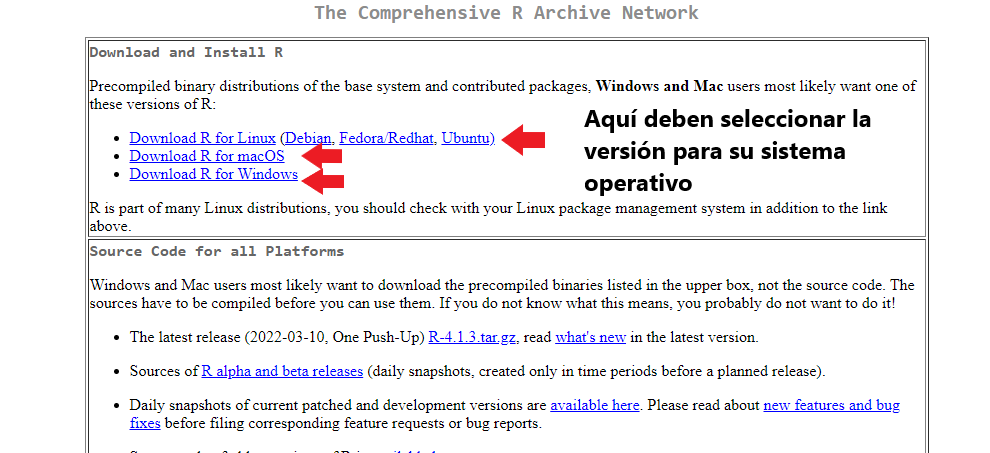
\includegraphics[keepaspectratio,width=\textwidth, height=.8\textheight]{input/img/img1_1.png}
\caption{R Paso 1}\label{rpaso1}
\end{figure}

\begin{itemize}
\tightlist
\item
  Para este ejemplo usaremos Windows.
\end{itemize}
\end{frame}

\begin{frame}{Descargando R base}
\phantomsection\label{descargando-r-base-2}
\begin{figure}[H]
\centering
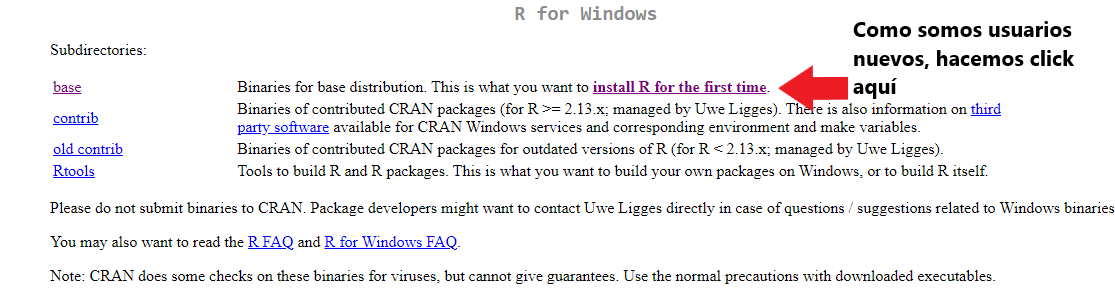
\includegraphics[keepaspectratio,width=\textwidth, height=.8\textheight]{input/img/img1_2.png}
\caption{R Paso 2}\label{rpaso2}
\end{figure}
\end{frame}

\begin{frame}{Descargando R base}
\phantomsection\label{descargando-r-base-3}
\begin{figure}[H]
\centering
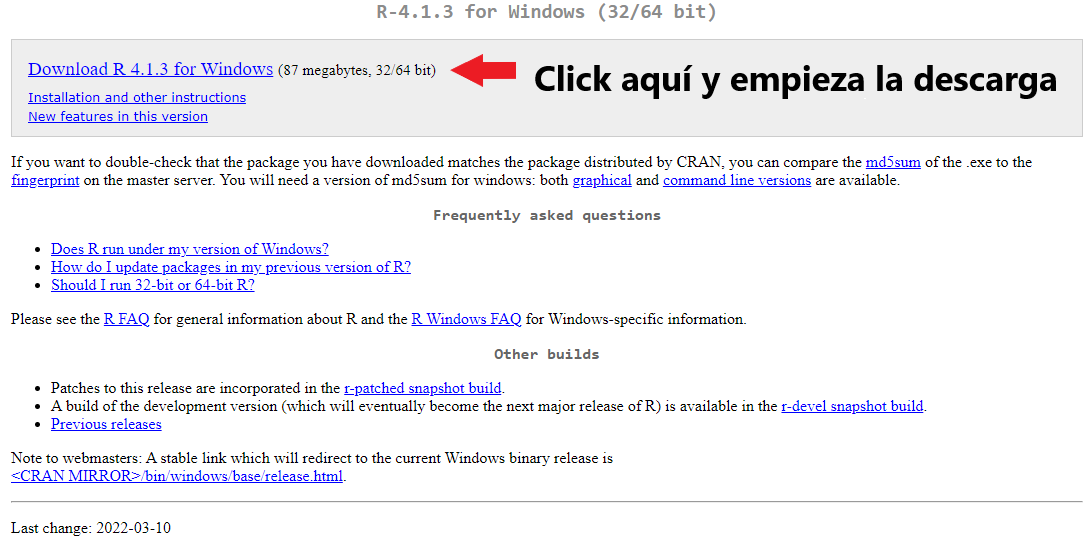
\includegraphics[keepaspectratio,width=\textwidth, height=.8\textheight]{input/img/img1_3.png}
\caption{R Paso 3}\label{rpaso3}
\end{figure}
\end{frame}

\begin{frame}{Descargando R base}
\phantomsection\label{descargando-r-base-4}
\begin{itemize}
\tightlist
\item
  Ya con R base descargado, procedemos a la instalación.
\end{itemize}

\begin{figure}[H]
\centering
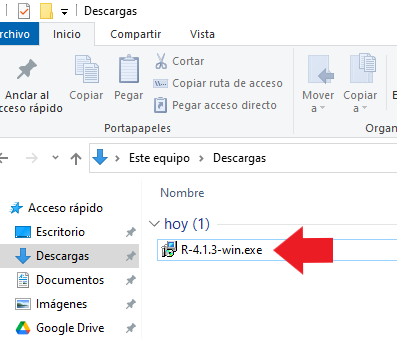
\includegraphics[keepaspectratio,width=\textwidth, height=.6\textheight]{input/img/img1_4.png}
\caption{R Paso 4}\label{rpaso4}
\end{figure}
\end{frame}

\begin{frame}{Instalando R base}
\phantomsection\label{instalando-r-base}
\begin{itemize}
\tightlist
\item
  Para la instalación no necesitamos aplicar ninguna configuración
  especial, simplemente instalar el programa.
\end{itemize}
\end{frame}

\section{RStudio}\label{rstudio}

\begin{frame}{RStudio}
\begin{itemize}
\item
  Una vez instalado R base, necesitamos un segundo software, RStudio.
\item
  Utilizaremos RStudio como interfaz del software R base.
\item
  Comentaremos sus características cuando ya esté instalado.
\item
  Lo descargamos aquí: \url{https://www.rstudio.com/}
\end{itemize}
\end{frame}

\begin{frame}{Descargando RStudio}
\phantomsection\label{descargando-rstudio}
\begin{figure}[H]
\centering
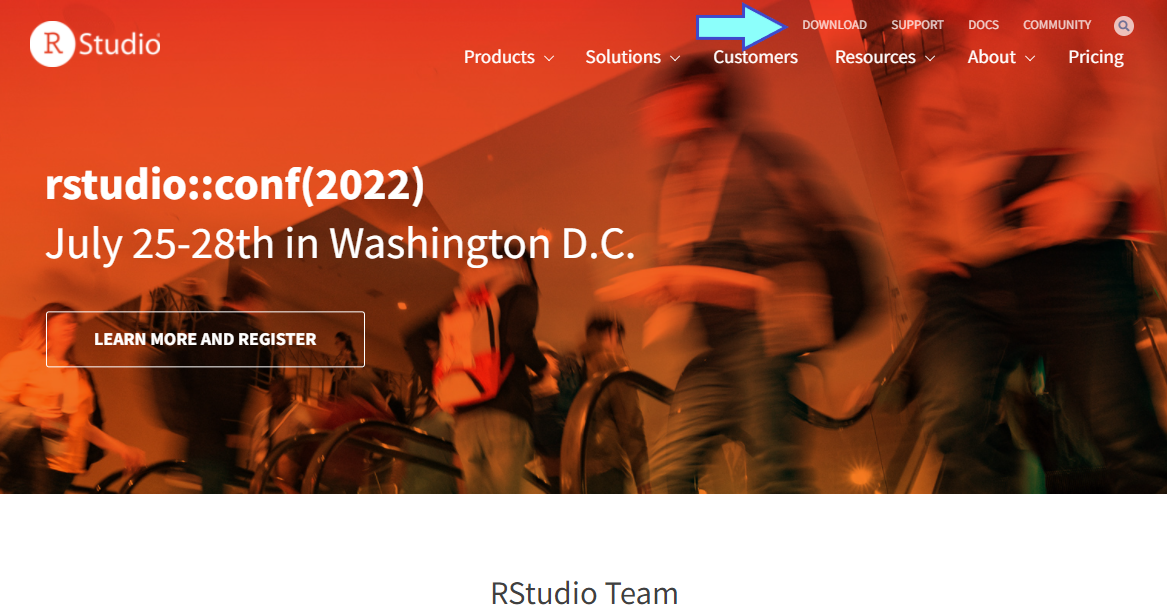
\includegraphics[keepaspectratio,width=\textwidth, height=.8\textheight]{input/img/img1_5.png}
\caption{RStudio Paso 1}\label{rstudiopaso1}
\end{figure}
\end{frame}

\begin{frame}{Descargando RStudio}
\phantomsection\label{descargando-rstudio-1}
\begin{figure}[H]
\centering
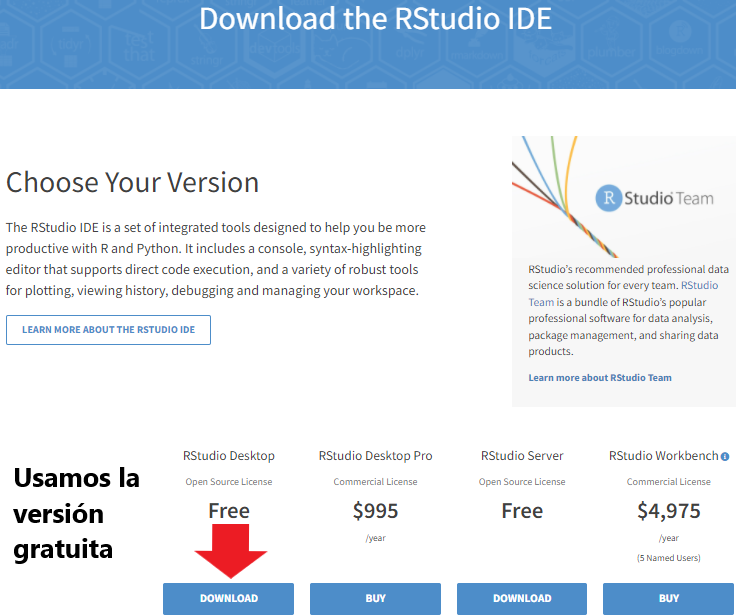
\includegraphics[keepaspectratio,width=\textwidth, height=.8\textheight]{input/img/img1_6.png}
\caption{RStudio Paso 2}\label{rstudiopaso2}
\end{figure}
\end{frame}

\begin{frame}{Descargando RStudio}
\phantomsection\label{descargando-rstudio-2}
\begin{figure}[H]
\centering
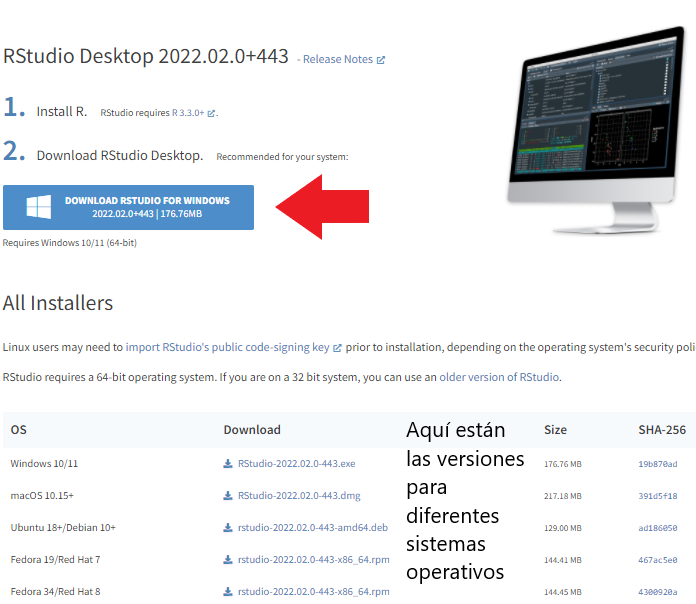
\includegraphics[keepaspectratio,width=\textwidth, height=.6\textheight]{input/img/img1_7.png}
\caption{RStudio Paso 3}\label{rstudiopaso3}
\end{figure}

\begin{itemize}
\tightlist
\item
  Para este ejemplo usaremos Windows.
\end{itemize}
\end{frame}

\begin{frame}{Descargando RStudio}
\phantomsection\label{descargando-rstudio-3}
\begin{figure}[H]
\centering
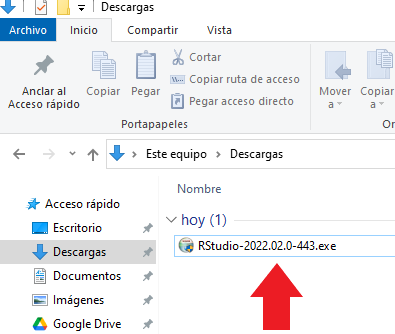
\includegraphics[keepaspectratio,width=\textwidth, height=.8\textheight]{input/img/img1_8.png}
\caption{RStudio Paso 4}\label{rstudiopaso4}
\end{figure}
\end{frame}

\begin{frame}{Instalando RStudio}
\phantomsection\label{instalando-rstudio}
\begin{itemize}
\tightlist
\item
  No necesitamos aplicar ninguna configuración especial, sólo instalar
  el software.
\end{itemize}
\end{frame}

\section{Usando RStudio}\label{usando-rstudio}

\begin{frame}{Usando RStudio}
\begin{itemize}
\tightlist
\item
  Cuando abramos RStudio veremos 4 ventanas o pestañas.
\end{itemize}

\begin{figure}[H]
\centering
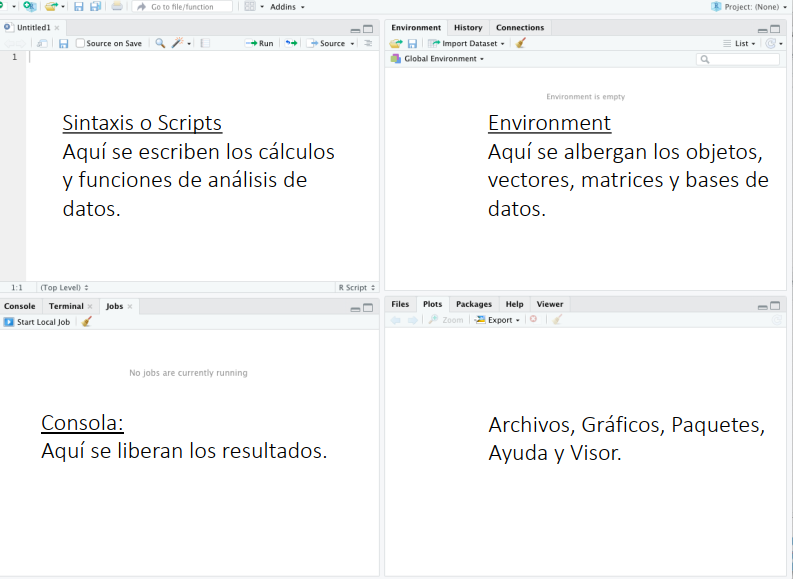
\includegraphics[keepaspectratio,width=\textwidth, height=.7\textheight]{input/img/img1_9.png}
\caption{Usando RStudio (imagen prof. Ignacio Cabib)}\label{rstudiousando1}
\end{figure}
\end{frame}

\begin{frame}{Consola y hoja de sintaxis}
\phantomsection\label{consola-y-hoja-de-sintaxis}
\begin{columns}[t]
    \begin{column}{.65\textwidth}
      \adjincludegraphics[width=1.025\linewidth, valign=t]{input/img/img1_10.png}
    \end{column}
    \begin{column}{.5\textwidth}
      \begin{itemize}
        \item En la \textbf{consola \textcolor{red}{(1)}} podemos escribir código para realizar nuestros análisis y ver nuestros resultados.
        \item La ventaja de usar la ventana de \textbf{sintaxis o scripts \textcolor{cyan}{(2)}} es que podemos guardar nuestro código en un archivo y ``correrlo'' desde ahí.
      \end{itemize}
    \end{column}
  \end{columns}
\end{frame}

\begin{frame}{Consola y hoja de sintaxis}
\phantomsection\label{consola-y-hoja-de-sintaxis-1}
\begin{columns}[t]
    \begin{column}{.65\textwidth}
      \adjincludegraphics[width=1.025\linewidth, valign=t]{input/img/img1_10.png}
    \end{column}
    \begin{column}{.5\textwidth}
      \begin{itemize}
        \item Al guardar nuestro código en una \textbf{hoja de sintaxis (o script) \textcolor{cyan}{(2)}}, podemos hacer análisis sin tener que escribirlos manualmente en la consola.
        \item Además, guardar el código permite que nuestros análisis sean reproducibles, de modo que otros investigadores puedan revisarlos.
      \end{itemize}
    \end{column}
  \end{columns}
\end{frame}

\begin{frame}{Consola y hoja de sintaxis}
\phantomsection\label{consola-y-hoja-de-sintaxis-2}
\begin{columns}[t]
    \begin{column}{.65\textwidth}
      \adjincludegraphics[width=1.025\linewidth, valign=t]{input/img/img1_10.png}
    \end{column}
    \begin{column}{.5\textwidth}
      \begin{itemize}
        \item Hacer análisis reproducibles y transparentes es un gran logro hacia una mejor investigación científica.
        \item En términos prácticos, el uso de código es de las cosas que más nos aparta de software como Excel y lo que para algunas personas puede resultar más incómodo al principio.
      \end{itemize}
    \end{column}
  \end{columns}
\end{frame}

\begin{frame}{Environment}
\phantomsection\label{environment}
\begin{columns}[t]
    \begin{column}{.65\textwidth}
      \adjincludegraphics[width=1.025\linewidth, valign=t]{input/img/img1_11.png}
    \end{column}
    \begin{column}{.5\textwidth}
      \begin{itemize}
        \item La ventana superior a la derecha se denomina \textbf{environment \textcolor{violet}{(3)}}.
        \item R se define como un ''lenguaje de programación orientada a objetos''.
      \end{itemize}
    \end{column}
  \end{columns}
\end{frame}

\begin{frame}{Environment}
\phantomsection\label{environment-1}
\begin{columns}[t]
    \begin{column}{.5\textwidth}
      \adjincludegraphics[width=1.025\linewidth, valign=t]{input/img/img1_11.png}
    \end{column}
    \begin{column}{.65\textwidth}
      \begin{itemize}
        \item Mediante el código ingresado en la sintaxis o la consola iremos ''creando'' objetos, que luego serán ''almacenados'' en el \textbf{environment \textcolor{violet}{(3)}}.
        \item Estos objetos pueden ser bases de datos, pero también valores (números, texto, etc.), análisis, tablas, gráficos, etc.
        \item Esos objetos podrán ser utilizados a su vez para realizar nuevas operaciones y crear nuevos objetos (que también se pueden almacenar en el environment).
      \end{itemize}
    \end{column}
  \end{columns}
\end{frame}

\begin{frame}{Visor de gráficos}
\phantomsection\label{visor-de-gruxe1ficos}
\begin{columns}[t]
    \begin{column}{.65\textwidth}
      \adjincludegraphics[width=1.025\linewidth, valign=t]{input/img/img1_12.png}
    \end{column}
    \begin{column}{.5\textwidth}
      \begin{itemize}
        \item Finalmente, la ventana inferior-derecha, el \textbf{visor de gráficos \textcolor{green}{(4)}}, servirá principalmente para ver gráficos producidos mediante nuestro código.
        \item También tiene herramientas para administrar archivos y ''paquetes'' (ya veremos qué son más adelante), pero en general se usa más para mirar gráficos.
      \end{itemize}
    \end{column}
  \end{columns}
\end{frame}

\begin{frame}{Tranquilidad}
\phantomsection\label{tranquilidad}
\begin{itemize}
\item
  Esto puede parecer muy árido e intimidante a primera vista, pero al
  familiarizarse con el software se irá volviendo mucho más intuitivo.
\item
  Haremos ejercicios para utilizar todas las ventanas correctamente.
\end{itemize}
\end{frame}

\end{document}
